\section{Languages without Optimal Proof Systems} 
\subsection{Languages without Optimal Proof Systems}

\begin{frame}
  \frametitle{Languages without Optimal Proof Systems}
  
  \begin{theorem}
    There exists a language \(L \in \coNTIME(2^n)\), that does not possess an optimal proof system.
  \end{theorem}
\end{frame}

\subsection{Proof}

\begin{frame}
  \frametitle{Proof Overview}

  \begin{enumerate}
   \item<1-> Let \(f_1, f_2, ...\) be an enumeration of all polynomial time functions
   \item<2-> \(L_i = 0^i10^*\) \\
              \onslide<3-> Let \(L_i'\) be the language of all strings \(L_i\) without any ``short'' \(f_i\)-proof \\
              \onslide<4-> \(L = \bigcup_i L_i' \in \coNTIME(2^n)\)
   \item<5-> We will show that for \(L\)-proof-systems \(f_i\) it holds \(L_i' = L_i\). As a consequence, there are only long \(f_i\)-proofs for \(L_i' \subset L\)
   \item<6-> This will contradict to the assumption, that \(f_i\) is an optimal proof system for \(L\).
  \end{enumerate}
\end{frame}

\begin{frame}
  \frametitle{Enumerating \(\FP\)}

  \begin{columns}
    \column{.7\textwidth}
      \begin{itemize}
        \item<2-> Gödel: \(M_1, M_2, ...\)
        \item<3-> We define \(M_1', M_2', ...\) as the \(M_i\) with a clock that stops the calculation after \(n^i + i\) steps
        \item<4-> Let \(f_i\) the function calculated by \(M_i\)
        \item<5-> As for unbounded \(i\), the runtime \(n^i + i\) is unbounded, we obtain all \(\FP\) functions
      \end{itemize}

    \column{.3\textwidth}
      \begin{figure}
        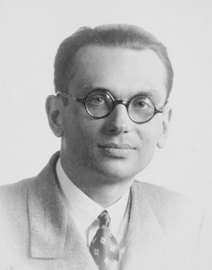
\includegraphics[width=\textwidth]{Presentation/Images/KurtGoedel.jpg}
        \caption{Kurt Gödel \\ 1906 -- 1978}
      \end{figure}
  \end{columns}
\end{frame}

\begin{frame}
  \frametitle{Construction of \(L\)}

  \begin{itemize}
    \item<1-> \(L_i = 0^i10^*\)
    \item<2-> take \(x \in L_i'\), that do not have \(f_i\)-proofs
              \[L_i' = \{ x \in L_i : \forall_{y \in \Sigma^*} |y|^{2i} \leq 2^{|x|} \implies f_i(y) \neq x \}\]
    \item<3-> union
              \[L = \bigcup_{i>0} L_i' \]
  \end{itemize}
\end{frame}

\begin{frame}
  \frametitle{\(L\) is member of \(\coNTIME(2^n)\)}

  \begin{itemize}
   \item<2-> As \(L \in \coNTIME(2^n) \Leftrightarrow \overline{L} \in \NTIME(2^n)\), we will analyze the complexity of \(\overline{L}\).
   \item<3-> \(\overline{L} = \) \onslide<4-> \( \overline{ \bigcup_{i>0} L_i' } = \) \onslide<5-> \( \bigcap_{i>0} \overline{L_i'}\)
   \item<6-> claim: \( \bigcap_{i>0} \overline{L_i'} \in \NTIME(2^n)\)
  \end{itemize}

  \onslide<6->
  
  \(\overline{L_i'} = \{ x \in \Sigma^* : \alert<9>{ x \notin L_i } \vee \left( \alert<12>{ \exists_{y \in \Sigma^*} \left( |y|^{2i} \leq 2^{|x|} \right) } \wedge \alert<14>{ \left( f_i(y) = x \right) } \right)  \}\)

  \onslide<7-> Let \(x\) be an arbitrary string.

  \begin{itemize}
   \item<8-> Check, if \(x\) is member of any \(L_i\): \onslide<9-> \alert<9>{if not, then \(x \in \overline{L}\) }
   \item<10-> Otherwise, choose \(i^*\) such that \(x \in L_{i^*}\)
   \item<11-> \(x \in \overline{L_j'}\) for any \(j \neq i\)
   \item<12-> \alert<12>{for any \(y\) such that \(|y|^{2i} \leq 2^{|x|}\)}: \onslide<13-> calculate \(f_{i^*}(y)\). \onslide<14-> \alert<14>{If and only if there is a \(y\) such that \(f_{i^*}(y) = x\), then \(x \in \overline{L}\).}
  \end{itemize}

  \onslide<15>
\end{frame}


\begin{frame}
  \frametitle{A Property for Proof Systems of \(L\)}

  Recall \(L_i' = \{ x \in L_i : \forall_{y \in \Sigma^*} |y|^{2i} \leq 2^{|x|} \implies f_i(y) \neq x \}\) \\
  and \(\overline{L_i'} = \{ x \in \Sigma^* : x \notin L_i \vee \alert<6>{\left( \exists_{y \in \Sigma^*} |y|^{2i} \leq 2^{|x|} \wedge f_i(y) = x \right)}  \}\)
  
  \begin{itemize}
   \item<2-> any proof system of \(L\) is one of the \(f_i\)
   \item<3-> claim: for any \(f_i(\Sigma^*) = L\) it holds \(L_i = L_i'\)
  \end{itemize}

  \begin{itemize}
    \item<4-> let \(f_i\) be a proof system for \(L\)
    \item<5-> assume there is a \(x = 0^i1z \in L_i\) that \alert<8>{is not a member of \(L_i'\)}
    \item<6-> \alert<6>{then, there is a \(y\) such that \(y^{2i} \leq 2^{|x|}\) and \(f_i(y) = x\)}
    \item<7-> Hence, \(y\) is a \(f_i\)-proof for \(x\). It follows that \(x \in L\), and therefore \alert<8>{\(x \in L_i'\)}. \onslide<8-> This is a contradiction.
  \end{itemize}
\end{frame}

\begin{frame}
  \frametitle{These results contradict the existence of an optimal proof system for \(L\)}

  Recall \(L_i' = \{ x \in L_i : \forall_{y \in \Sigma^*} |y|^{2i} \leq 2^{|x|} \implies f_i(y) \neq x \}\).

  \begin{itemize}
   \item<1-> Let \(f_i\) be an optimal proof system for \(L\)
   \item<2-> Let \(g\) be defined by
         \(g(bx) =
           \begin{cases}
             f_i(x) & (b=0) \\
             x      & (b = 1 \text{ and } x=0^i10^* \in L_i = L_i') 
           \end{cases}\)
   \item<3-> \(g\) is a proof system for \(L\)
   \item<4-> as \(f_i\) is optimal, there is a \(f^*\), such that \(f_i(f^*(x)) = g(x)\). \(f^*\) is polynomial bounded: \(|f^*(x)| \leq p(|x|)\)
   \item<5-> for any \(x\) of \(L_i'\), such that \(p(|1x|)^{2i} \leq 2^{|x|}\).
   \item<6-> \(1x\) is a \(g\)-proof for \(x\): \(g(1x) = x\)
   \item<7-> For \(y = f^*(1x)\) it holds \(|y| = |f^*(1x)| \leq p(|1x|) \leq p(|1x|)^{2i} \leq 2^{|x|}\).
   \item<8-> By Definition of \(L_i'\): \(f_i(y) \neq x\), hence \(y = f^*(1x)\) is no \(f_i\)-proof for \(x\)
   \item<9-> This is a contradiction \onslide<10-> \(\square\)
  \end{itemize}

\end{frame}

